\documentclass[12pt]{ociamthesis}  % default square logo 
%\documentclass[12pt,beltcrest]{ociamthesis} % use old belt crest logo
%\documentclass[12pt,shieldcrest]{ociamthesis} % use older shield crest logo

%load any additional packages
\usepackage{amssymb}
\usepackage{listings}
\usepackage{float}
\usepackage{color}
 
\definecolor{codegreen}{rgb}{0,0.6,0}
\definecolor{codegray}{rgb}{0.5,0.5,0.5}
\definecolor{codepurple}{rgb}{0.58,0,0.82}
\definecolor{backcolour}{rgb}{0.95,0.95,0.92}
 
\lstdefinestyle{mystyle}{
    backgroundcolor=\color{backcolour},   
    commentstyle=\color{codegreen},
    keywordstyle=\color{magenta},
    numberstyle=\tiny\color{codegray},
    stringstyle=\color{codepurple},
    basicstyle=\footnotesize,
    breakatwhitespace=false,         
    breaklines=true,                 
    captionpos=b,                    
    keepspaces=true,                 
    numbers=left,                    
    numbersep=5pt,                  
    showspaces=false,                
    showstringspaces=false,
    showtabs=false,                  
    tabsize=2,
    language=python
}
 
\lstset{style=mystyle}
%input macros (i.e. write your own macros file called mymacros.tex 
%and uncomment the next line)
%\include{mymacros}

\title{Tugas \\[1ex]     %your thesis title,
        Kecerdasan Buatan}   %note \\[1ex] is a line break in the title

\author{Heriyanto}             %your name
\college{1184023\\[5ex]
Applied Bachelor of Informatics Engineering}  %your college

%\renewcommand{\submittedtext}{change the default text here if needed}
\degree{Politeknik Pos Indonesia}     %the degree
\degreedate{Bandung 2021}         %the degree date

%end the preamble and start the document
\begin{document}

%this baselineskip gives sufficient line spacing for an examiner to easily
%markup the thesis with comments
\baselineskip=18pt plus1pt

%set the number of sectioning levels that get number and appear in the contents
\setcounter{secnumdepth}{3}
\setcounter{tocdepth}{3}


\maketitle                  % create a title page from the preamble info
%\begin{dedication}
`Jika Kamu tidak dapat menahan lelahnya belajar, \\
Maka kamu harus sanggup menahan perihnya Kebodohan.'\\ 
~Imam Syafi'i~\\
\end{dedication}        % include a dedication.tex file
%\begin{acknowledgements}
Pertama-tama kami panjatkan puji dan syukur kepada Allah SWT yang telah memberikan rahmat dan hidayah-Nya sehingga Buku Pedoman Tingkat Akhir ini dapat diselesaikan.
\end{acknowledgements}   % include an acknowledgements.tex file
\begin{abstract}
	Buku Pedoman ini dibuat dengan tujuan memberikan acuan, bagi mahasiswa Tingkat Akhir dan dosen
	Pembimbing. Pada intinya buku ini menjelaskan secara lengkap tentang Standar pengerjaan Intership  dan 
	Tugas Akhir
	di Program Studi D4 Teknik Informatika, dan juga mengatur mekanisme, teknik penulisan, serta
	penilaiannya.Dengan demikian diharapkan semua pihak yang terlibat dalam aktivitas Bimbingan Mahasiswa Tingkat Akhir
	berjalan lancar dan sesuai dengan standar.
\end{abstract}          % include the abstract

\begin{romanpages}          % start roman page numbering
\tableofcontents            % generate and include a table of contents
\listoffigures              % generate and include a list of figures
\end{romanpages}            % end roman page numbering

%now include the files of latex for each of the chapters etc
\chapter{Mengenal Kecerdasan Buatan dan Scikit-Learn}
\section{Teori}
\subsection{Definisi Kecerdasan Buatan}
\hfill\break
Kecerdasan buatan atau artificial intelligence (AI) menurut beberapa pakar adalah sebagai berikut:
\begin{enumerate}
	\item Schalkoff (1990): AI adalah bidang studi yang mencoba meniru dan menerangkan perilaku cerdas yang dilakukan oleh manusia dalam bentuk proses komputasi.
	\item Rich dan Knight (1991): AI adalah studi tentang cara membuat komputer melakukan sesuatu yang sampai saat ini orang dapat melakukannya lebih baik.
	\item Luger dan Stubblefield (1993): AI adalah cabang ilmu komputer yang berhubungan dengan otomasi perilaku yang cerdas.
\end{enumerate}

\noindent
Jadi dapat disimpulkan kecerdasan buatan atau artificial intelligence (AI) merupakan salah satu bagian ilmu komputer yang membuat mesin (komputer) dapat melakukan pekerjaan seperti dan sebaik yang dilakukan oleh manusia. Seperti yang kita tahu pada awal diciptakannya, komputer hanya difungsikan sebagai alat hitung saja. Namun seiring dengan perkembangan jaman, maka peran komputer semakin mendominasi kehidupan umat manusia. Komputer tidak lagi sekedar digunakan sebagai alat hitungn namun diharapkan untuk dapat diberdayakan untuk mengerjakan segala sesuatu yang bisa dikerjakan oleh manusia.

\subsection{Sejarah dan Perkembangan Kercerdasan Buatan}
\hfill\break
Istilah AI pertama kali dikemukakan pada tahun 1956 dikonferensi Darthmouth. Sejak saat itu AI terus dikembangkan sebab berbagai penelitian mengenai teori-teori dan prinsip-prinsipnya juga terus berkembang. Meskipun istilah AI baru muncul tahun 1956, tetapi teori-teori mengarah ke AI sudah muncul sejak tahun 1941. Berikut ini tahapan-tahapan sejarah perkembangan AI:
\begin{enumerate}
	\item Era Komputer Elektronik (1941)
	\hfill\break
	Pada tahun 1941 telah ditemukan alat penyimpanan dan pemrosesan informasi. Penemuan tersebut dinamakan komputer elektronik yang dikembangkan di USA dan Jerman. Komputer pertama ini memerlukan ruangan yang luas dan ruang AC yang terpisah. Saat itu komputer meibatkan konfigurasi ribuan kabel untuk menjalankan suatu program. Hal ini sangat merepotkan bagi para programmer. Pada tahun 1949, berhasil dibuat komputer yang mampu menyimpan program sehingga membuat pekerjaan untuk memasukkan program menjadi lebih mudah. Penemuan ini menjadi dasar pengembangan program yang mengarah ke AI.

	\item Masa Persiapan AI (1943–1956)
	\hfill\break
	Pada tahun 1943, Warren McCulloch dan Walter Pitts mengemukakan tiga hal: pengetahuan fisiologi dasar dan fungsi sel syaraf dalam otak, analisis formal tentang logika proporsi (propositional logic), dan teori komputasi turing. Mereka berhasil membuat suatu model syaraf tiruan (artificial neuron) di mana setiap neuron digambarkan sebagai on dan off. Mereka menunjukkan bahwa setiap fungsi dapat dihitung dengan suatu jaringan sel syaraf dan bahwa semua hubungan logis dapat diimplementasikan dengan struktur jaringan yang sederhana.
	\noindent
	Pada tahun 1950, Norbert Wiener mebuat penelitian mengenai prinsip-prinsip teori feedback. Contoh yang terkenal adalah thermostat. Penemuan ini juga merupakan awal perkembangan AI. Pada tahun 1956, John McCarthy (yang setelah lulus dari Princeton kemudian melanjutkan ke Dartmouth College) meyakinkan Minsky, Claude Shannon dan Nathaniel Rochester untuk membantunya melakukan penelitian dalam bidang Automata, jaringan sel syaraf dan pembelajaran intelejensia. Mereka mengerjakan proyek ini selama dua bulan di Dartmouth. Hasilnya adalah program yang mampu ber-pikir non-numerik dan menyelesaikan masalah pemikiran, yang dinamakan Principia Mathematica. Hal ini menjadikan McCarthy disebut sebagai Father of AI (Bapak AI).

	\item Awal Perkembangan AI (1952–1969)
	\hfill\break
	Pada tahun-tahun pertama pengembangannya, AI mengalami banyak kesuksesan. Diawali dengan kesuksesan Newell dan Simon dengan sebuah program yang disebut General Problem Solver. Program ini dirancang untuk memulai penyelesaian masalah secara manusiawi. Pada tahun 1958, McCarthy di MTT Lab Memo No. 1 mendefinisikan bahasa pemrograman tingkat tinggi yaitu LISP, yang sekarang mendominasi pembuatan program-program AI. Kemudian, McCarthy membuat program yang dinamakan Programs With Common Sense. Di dalam program tersebut, dibuat rancangan untuk menggunakan pengetahuan dalam mencari solusi. Pada tahun 1959, Nathaniel Rochester dari IBM dan mahasiswa-mahasiswanya mengeluarkan program AI Geometry Theorm Prover. Program ini dapat membuktikan suatu teorema menggunakan axioma-axioma yang ada. Pada tahun 1963, program yang dibuat James Slagle mampu menyelesaikan masalah integral tertutup untuk mata kuliah kalkulus. Pada tahun 1968, program analogi buatan Tom Evan menyelesaikan masalah analogi geometris yang ada pada tes IQ.

	\item Perkembangan AI Melambat (1966–1974)
	\hfill\break
	Prediksi Herbert Simon pada tahun 1957 yang menyatakan bahwa AI akan menjadi ilmu pengetahuan yang akan berkembang dengan pesat ternyata meleset. Pada 10 tahun kemudian, perkembangan AI melambat. Hal ini disebabkan adanya 3 kesulitan utama yang dihadapi AI, yaitu:
	\begin{enumerate}
		\item Masalah pertama: program-program AI yang bermunculan hanya mangandung sedikit atau bahkan tidak mengandung sama sekali pengetahuan (knowledge) pada subjeknya. Program-program AI berhasil hanya karena manipulasi sintetis yang sederhana. Sebagai contoh adalah Weizenbaum’s ELIZA program (1965) yang dapat melakukan percakapan serius pada berbagai topik, sebenarnya hanyalah peminjaman dan manipulasi kalimat-kalimat yang diketikkan oleh manusia.
		\item Masalah kedua: banyak masalah yang harus diselesaikan oleh AI. Karena terlalu banyaknya masalah yang berkaitan, maka tidak jarang banyak terjadi kegagalan pada pembuatan program AI.
		\item Masalah ketiga: ada beberapa batasan pada struktur dasar yang digunakan untuk menghasilkan perilaku intelejensia. Sebagai contoh adalah pada tahun 1969 buku Minsky dan Papert Perceptrons membuktikan bahwa program-program perceptrons dapat mempelajari segala sesuatu, tetapi program-program tersebut hanya mempresentasikan sejumlah kecil saja. Sebagai contoh dua masukan perceptrons yang berbeda tidak dapat dilatihkan untuk mengenali kedua masukan yang berbeda tersebut.
	\end{enumerate}

	\item Sistem Berbasis Pengetahuan (1969–1979)
	\hfill\break
	Pengetahuan adalah kekuatan pendukung AI. Hal ini dibuktiikan dengan program yang dibuat oleh Ed Feigenbaum,Bruce Buchanan dan Joshua Lederberg yang membuat program untuk memecahkan masalah struktur molekul dari informasi yang didapatkan dari spectometer massa. Program ini dinamakan Dendral programs yang berfokus pada segi pengetahuan kimia. Dari segi diagnosis media juga sudah ada yang menemukannya, yaitu Saul Amarel dalam proyek computer in biomedicine. Proyek ini diawali dari keinginan untuk mendapatkan diagnosa penyakit berdasarkan pengetahuan yang ada pada mekanisme penyebab proses penyakit.

	\item AI Menjadi Sebuah Industri (1980–1988)
	\hfill\break
	Industrialisasi AI diawali dengan ditemukannya expert system (sistem pakar) yang dinamakan R1 yang mampu mengkonfigurasi sistem-sistem komputer baru. Program tersebut mulai dioperasikan di Digital Equipment Corporation(DEC), McDermott, pada tahun 1982. Pada tahun 1986, program ini telah berhasil menghemat US\$40 juta per tahun. Pada tahun 1988, kelompok AI di DEC menjalankan 40 sistem pakar. Hampir semua perusahaan besar di USA mempunyai divisi AI sendiri yang menggunakan ataupun mempelajari sistem pakar. Booming industri AI ini juga melibatkan perusahaan-perusahaan besar seperti Carnegie Group, Inference, Intellicorp, dan Technoledge yang menawarkan software tools untuk membangun sistem pakar. Perusahaan hardware seperti LISP dan Machines Inc., Texas Instruments, Symbolics, dan Xerox juga turut berperan dalam membangun workstation yang dioptimasi untuk pembangunan program LISP. Sehingga, perusahaan yang sejak tahun 1982 hanya menghasilkan beberapa juta US dolar per tahun meningkat menjadi 2 milyar US dolar per tahun pada tahun 1988.

	\item Kembalinya Jaringan Syaraf Tiruan (1986–Sekarang)
	\hfill\break
	Meskipun bidang ilmu komputer menolak jaringan syaraf tiruan setelah diterbitkannya buku "perceptrons" karangan Minsky dan Papert, tetapi para ilmuan masih mempelajari bidang ilmu tersebut dari sudut pandang yang lain yaitu fisika. Para ahli seperti Hopfield (1982) menggunakan teknik-teknik mekanika statistika untuk menganalisa sifat-sifat penyimpanan dan optimasi pada jaringan syaraf. Para ahli psikollogi, David Rumelhart dan Geoff Hinton, melanjutkan penelitian mengenai model syaraf pada memori. Pada tahun 1985-an sedikitnya empat kelompok riset menemukan kembali algoritma belajar propagasi balik (Back-Propagation Learning). Algoritma ini berhasil diimplementasikan kedalam bidang ilmu komputer dan psikologi.

\end{enumerate}

\subsection{Supervised Learning}
\hfill\break
Supervised Learning adalah pembelajaran yang memiliki label di tiap datanya. Label maksudnya adalah tag dari data yang ditambahkan dalam machine learning model. Contohnya gambar kucing di tag "kucing" di tiap masing masing image kucing dan gambar anjing di tag "anjing" di tiap masing gambar anjing. Machine learning kategori dapat berupa clasification ("anjing", "kucing", "beruang", dsb) dan regression ( berat badan, tinggi badan dsb). Supervised learning banyak digunakan dalam memprediksi pola dimana pola tersebut sudah ada contoh data yang lengkap, jadi pola yang terbentuk adalah hasil pembelajaran data lengkap tersebut. Tentunya jika kita memasukan data baru, setelah kita melakukan ETL (Extract Transform Load) maka kita mendapat info feature feature dari sample baru tersebut. Kemudian dari feature feature tersebut di compare dengan pattern clasification dari model yang didapat dari labeled data. Setiap label akan dicompare sampai selesai, dan yang memiliki percentage lebih banyak akan diambil sebagai prediksi akhir.

\begin{figure}[H]
	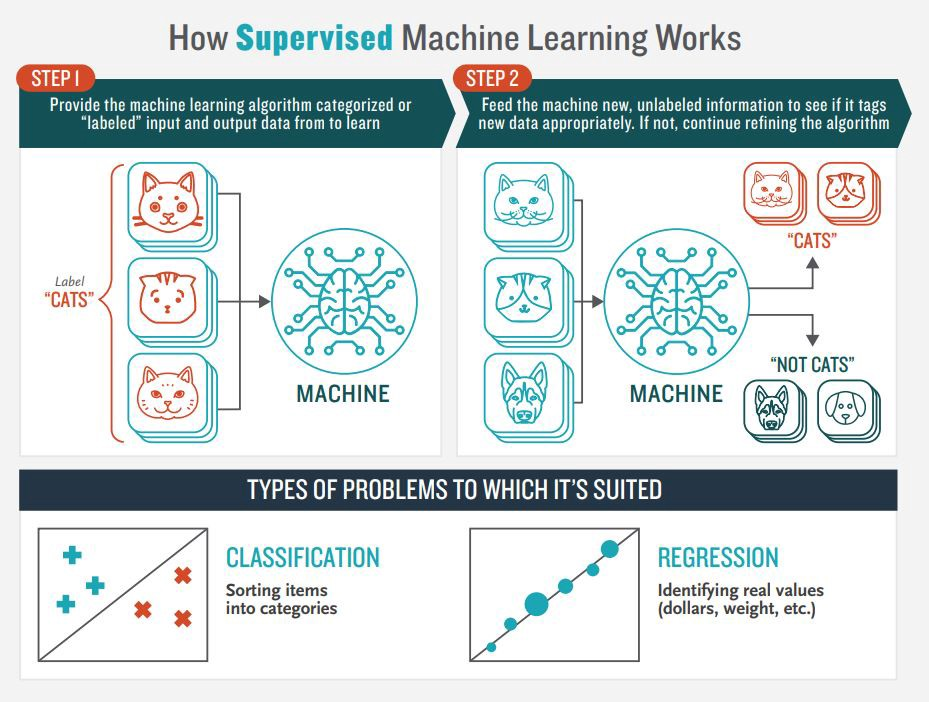
\includegraphics[width=1\textwidth]{figures/chapter1/supervisedlearning.jpeg}
	\centering
	\caption{Supervised Learning.}
\end{figure}
\noindent
Contoh algoritma yang digunakan pada supervised learning meliputi :
\begin{enumerate}
	\item Clasification (Categorical) and Regression (Numerical)
    \item Logistic Regression
    \item Model Ensemble
	\item Time series
\end{enumerate}

\subsection{Klasifikasi}
\hfill\break
Classification adalah tindakan untuk memberikan kelompok pada setiap keadaan. Setiap keadaan berisi sekelompok atribut, salah satunya adalah class attribute. Metode ini butuh untuk menemukan sebuah model yang dapat menjelaskan class attribute itu sebagai fungsi dari input attribute.

\noindent
Class adalah attribute CollegePlans yang berisi dua pernyataan, Yes dan No, perhatikan ini.
\noindent
Sebuah Classification Model akan menggunakan atribut lain dari kasus tersebut (input attribut; yaitu kolom IQ, Gender, ParentIncome, dan ParentEncouragement) untuk dapat menentukan pola (pattern) class (Output Attribute; yaitu Kolom CollegePlans yang berisi Yes atau No).
\noindent
Algoritma Data Mining yang membutuhkan variabel target untuk belajar (sampai mendapatkan rule / pola yang berlaku pada data tersebut) kita standarkan dengan sebuthan dengan Supervised Algorithm.
\noindent
Nah, yang termasuk kepada Classification Algorithm adalah Decision Trees, Neural Network dan Naives Bayes.
\subsection{Regresi}
\hfill\break
Metode Regression mirip dengan metode Classification, yang membedakannya adalah metode regression tidak bisa mencari pola yang dijabarkan sebagai class (kelas).
\noindent
Metoda regression bertujuan untuk mecari pola dan menentukan sebuah nilai numerik.
\noindent
Sebuah Teknik Linear Line-fitting sederhana adalah sebuah contoh dari Regression, dimana hasilnya adalah sebuah fungsi untuk menentukan hasil yang berdasarkan nilai dari input.
\noindent
Bentuk yang lebih canggih dari regression sudah mendukung input berupa kategori, jadi tidak hanya input berupa numerik. Teknik paling popular yang digunakan untuk regression adalah linear regression dan logistic regression. Teknik lain yang didukung oleh SQL Server Data mining adalah Regression Trees (bagian dari dari algoritma Microsoft Decission Trees) dan Neural Network.
\noindent
Regression digunakan untuk memecahkan banyak problem bisnis – contohnya untuk memperkirakan metode distribusi, kapasitas distribusi, musim dan untuk memperkirakan kecepatan angin berdasarkan temperatur, tekanan udara, dan kelembaban.
\subsection{Unsupervised Learning}
\hfill\break
Unsupervised learning memiliki keunggulan dari supervised learning. Jika supervised learning memiliki label sebagai dasar prediksi baik serta membuat clasification dan regression algorithm memungkinkan. Tetapi dalam realitanya, data real itu banyak yang tidak memiliki label. Label kebanyakan jika data sudah masuk ke ERP apapun bentuk ERPnya dan bagaimana kalo datanya berupa natural input seperti suara, gambar, dan video. Unsupervised learning tidak menggunakan label dalam memprediksi target feautures / variable. Melainkan menggunakan ke samaan dari attribut attribut yang dimiliki. Jika attribut dan sifat-sifat dari data data feature yang diekstrak memiliki kemirip miripan, maka akan dikelompok kelompokan (clustering). Sehingga hal ini akan menimbulkan kelompok kelompok (cluster). Jumlah cluster bisa unlimited. Dari kelompok kelompok itu model melabelkan, dan jika data baru mau di prediksi, maka akan dicocok kan dengan kelompok yang mirip mirip featurenya.
\begin{figure}[H]
	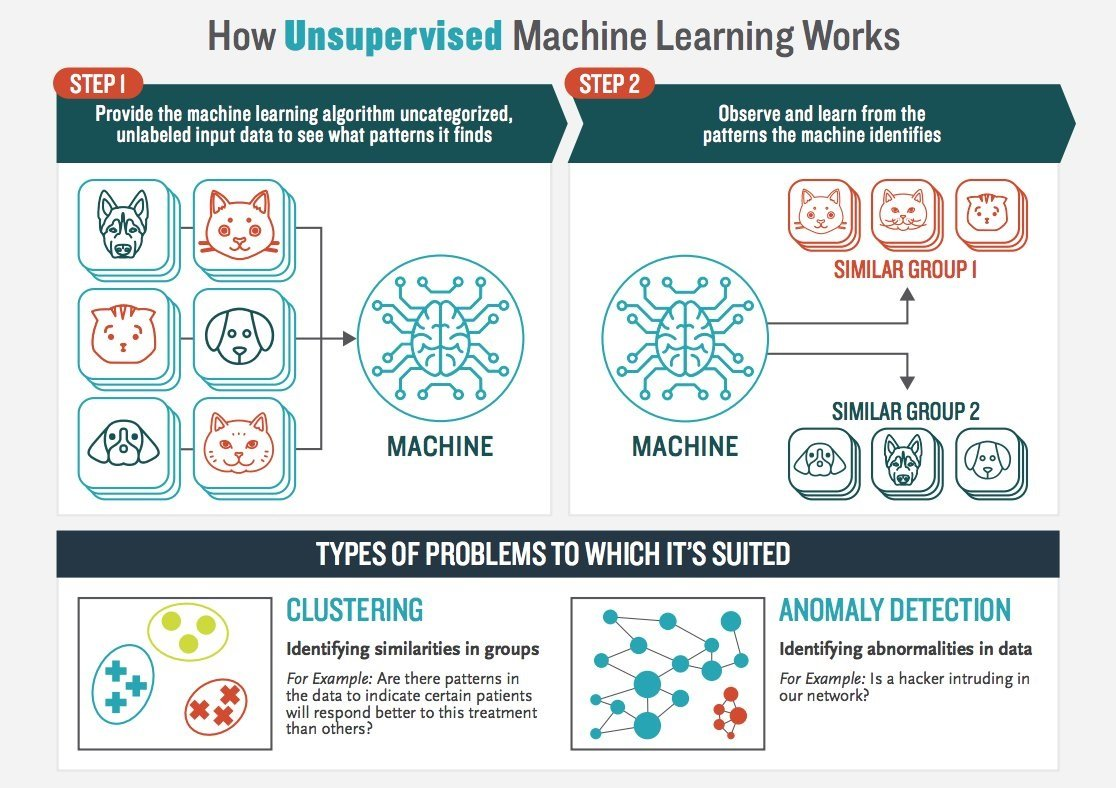
\includegraphics[width=1\textwidth]{figures/chapter1/unsupervisedlearning.jpg}
	\centering
	\caption{Unsupervised Learning.}
\end{figure}
\noindent
Tetapi unsupervise learning tidak memiliki outcome yang spesifik layaknya di supervise learning, hal ini dikarenakan tidak adanya ground truth / label dasar. Walaupun begitu, unsupervised learning masih dapat memprediksi dari ketidakadaan label dari kemiripan attribute yang dimilik data.
\noindent
Algoritma yang digunakan di unsupervised learning :
\begin{enumerate}
	\item Clustering
    \item Anomaly Detection
    \item Training Model
    \item Association Discovery
\end{enumerate}
\subsection{Data Set}
\hfill\break
Dataset adalah objek yang merepresentasikan data dan relasinya di memory. Strukturnya mirip dengan data di database. Dataset berisi koleksi dari datatable dan data relation.
\subsection{Training Set}
\hfill\break
Training set adalah bagian dataset yang kita latih untuk membuat prediksi atau menjalankan fungsi dari sebuah algoritma ML lainnya sesuai tujuannya masing-masing. Kita memberikan petunjuk melalui algoritma agar mesin yang kita latih bisa mencari korelasinya sendiri. 
\subsection{Testing Set}
\hfill\break
Test set adalah bagian dataset yang kita tes untuk melihat keakuratannya, atau dengan kata lain melihat performanya.


\section{Praktek}
\begin{enumerate}
	\item Instalasi  library  scikit  dari  anaconda,  mencoba  kompilasi  dan  uji  coba  ambil contoh kode dan lihat variabel explorer.
	
	\textbf{Instalasi Library Scikit-Learn melalui CMD }
	\begin{enumerate}
		\item Pertama masuk ke command prompt di menu start.
		\begin{figure}[H]
			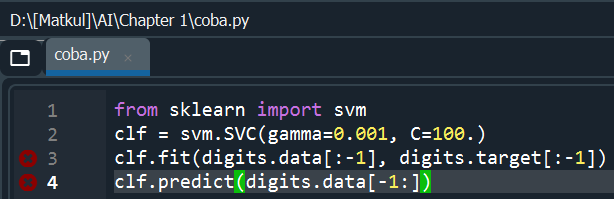
\includegraphics[width=1\textwidth]{figures/chapter1/praktek/1.PNG}
			\centering
			\caption{Instalasi Library Scikit-Learn.}
		\end{figure}
		\item Selanjutnya ketik "conda activate base" untuk masuk base anaconda.
		\item Kemudian ketik conda install scikit-learn.
		\item Lalu apabila sudah done , artinya library scikit sudah kita install
	\end{enumerate}

	\textbf{Mencoba Menggunakan Library scikit-Learn}
	\begin{enumerate}
		\item Pertama jalankan aplikasi Spyder.
		\item Kemudian buat file baru, lalu tambahkan kode berikut.
		\lstinputlisting[language=Python]{src/chapter1/Tugas1.py}
		\item Simpan dan jalankan.
		\item Hasil dari variabel explorernya sebagai berikut.
		\begin{figure}[H]
			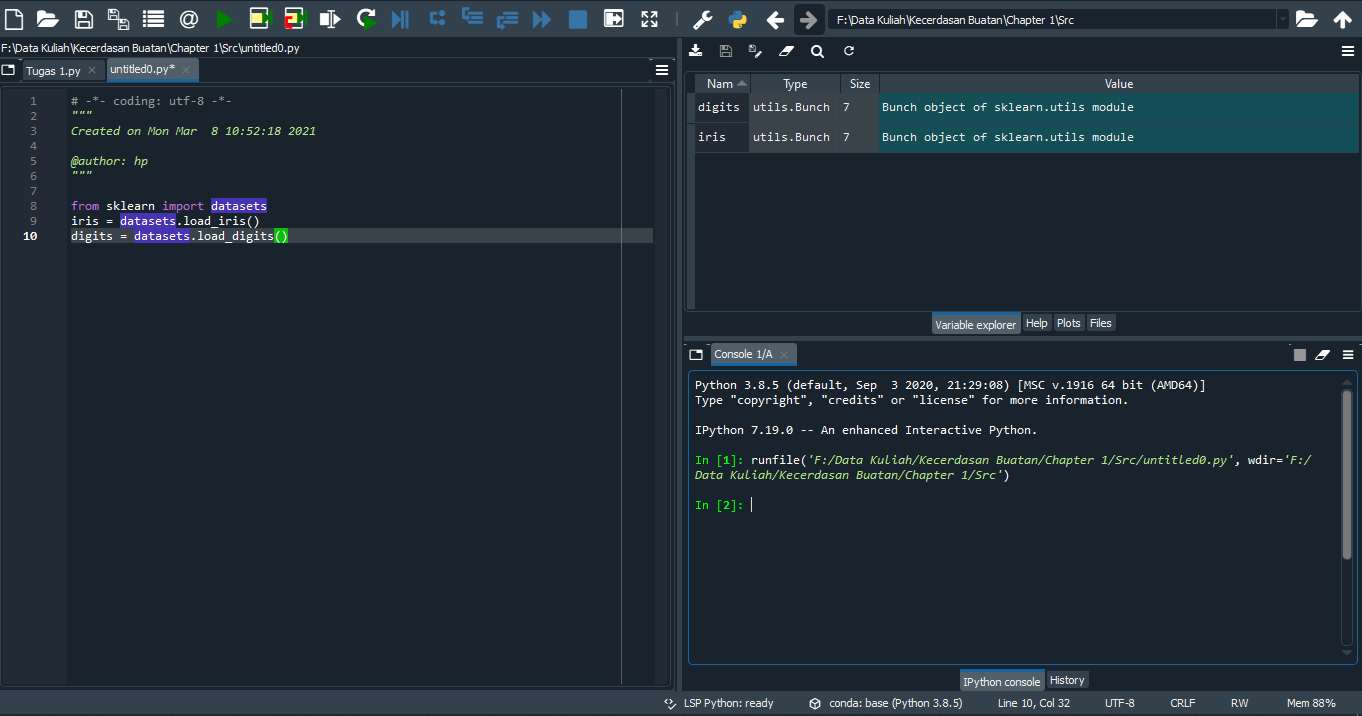
\includegraphics[width=1\textwidth]{figures/chapter1/praktek/contoh.PNG}
			\centering
			\caption{Variabel Explorer Library Scikit-Learn.}
		\end{figure}
	\end{enumerate}
	
	\item Mencoba Loading an example dataset, menjelaskan maksud dari tulisan terse-but dan mengartikan per baris.
	\lstinputlisting[firstline=3,lastline=7]{src/chapter1/Tugas1.py}
	
	Hasilnya akan seperti ini.
	\begin{figure}[H]
		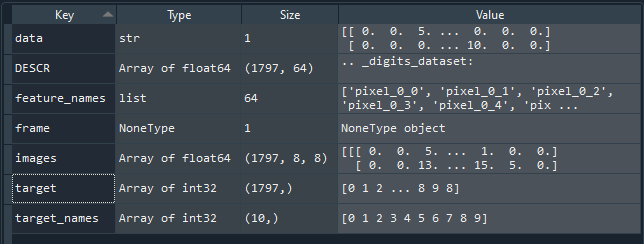
\includegraphics[width=7cm]{figures/chapter1/praktek/hasil1.PNG}
		\centering
		\caption{Hasil Loading an Example Dataset.}
	\end{figure}

	\item Mencoba  Learning  and  predicting,  menjelaskan  maksud  dari  tulisan  tersebut dan mengartikan per baris.
	\lstinputlisting[firstline=11,lastline=14]{src/chapter1/Tugas1.py}
	
	Hasilnya akan seperti ini.
	\begin{figure}[H]
		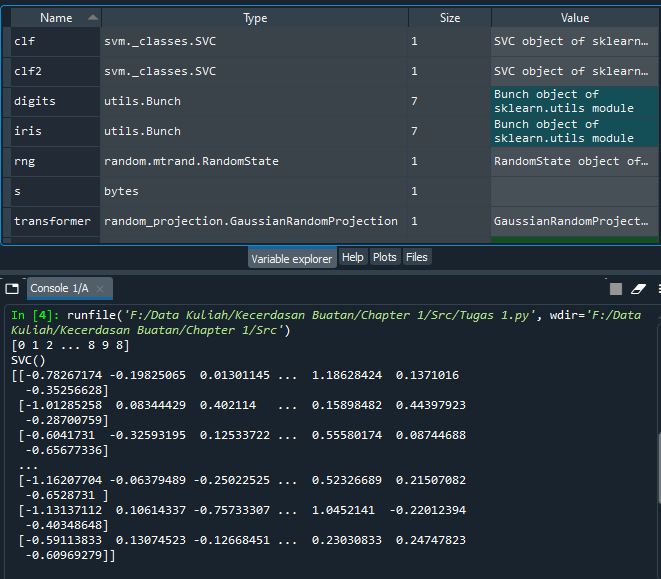
\includegraphics[width=7cm]{figures/chapter1/praktek/hasil2.PNG}
		\centering
		\caption{Hasil Learning and Predicting.}
	\end{figure}

	\item Mencoba Model persistence, menjelaskan maksud dari tulisan tersebut dan mengartikan per baris.
	\lstinputlisting[firstline=18,lastline=34]{src/chapter1/Tugas1.py}
	
	Hasilnya akan seperti ini.
	\begin{figure}[H]
		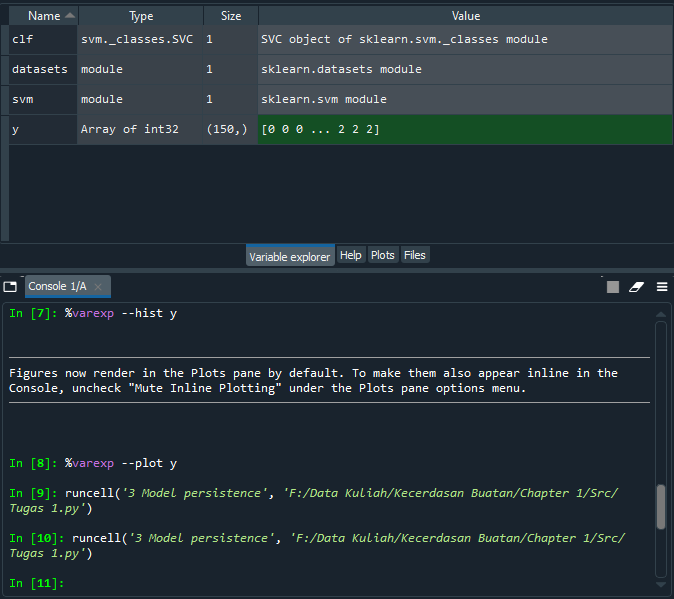
\includegraphics[width=8cm]{figures/chapter1/praktek/hasil3.PNG}
		\centering
		\caption{Hasil Model Persistence.}
	\end{figure}

	\item Mencoba Conventions, menjelaskan maksud dari tulisan tersebut dan mengartikan per baris.
	\lstinputlisting[firstline=35,lastline=49]{src/chapter1/Tugas1.py}
	
	Hasilnya akan seperti ini.
	\begin{figure}[H]
		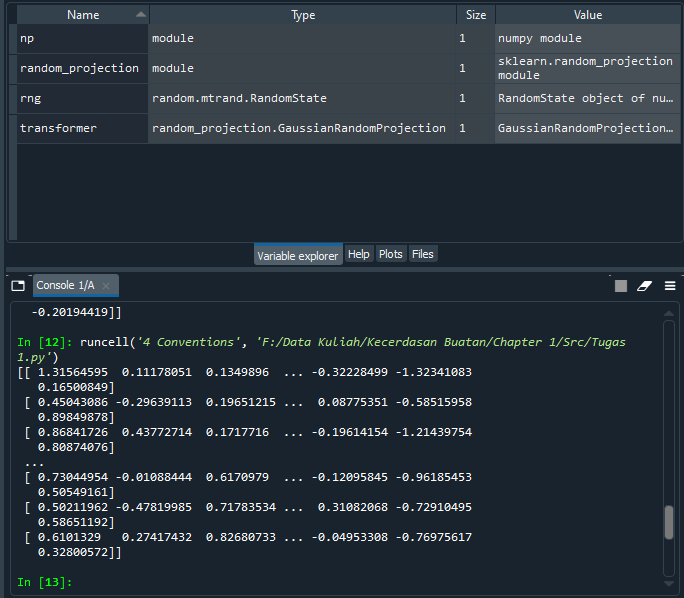
\includegraphics[width=10cm]{figures/chapter1/praktek/hasil4.PNG}
		\centering
		\caption{Hasil Conventions.}
	\end{figure}

\end{enumerate}

\section{Penanganan Error}
\begin{enumerate}
	\item Screenshoot error yang terjadi pada saat melakukan running syntax pada saat melakukan praktikum ini.
	\begin{itemize}
		\item Name Error dapat terjadi apabila terdapat kesalahan penulisan syntax, yang meliputi nama library, function etc.
		\hfill\break
		\begin{figure}[H]
			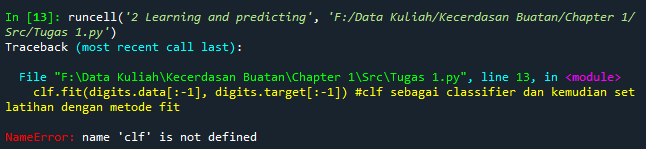
\includegraphics[width=10cm, height=3cm\textwidth]{figures/chapter1/error/error1.PNG}
			\centering
			\caption{Name Error.}
		\end{figure} \\ 

		\item Import Error
		\hfill\break
		\begin{figure}[H]
			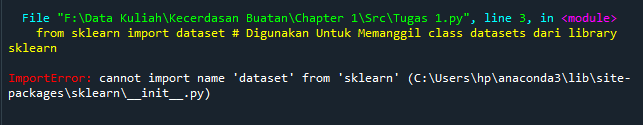
\includegraphics[width=1\textwidth]{figures/chapter1/error/error2.PNG}
			\centering
			\caption{Import Error.}
		\end{figure}
		\item Syntax Error
		\hfill\break
		\begin{figure}[H]
			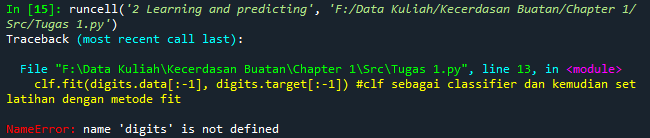
\includegraphics[width=1\textwidth]{figures/chapter1/error/error3.PNG}
			\centering
			\caption{Syntax Error.}
		\end{figure}
	\end{itemize}
	\item Tuliskan kode eror dan jenis errornya.
	\begin{itemize}
		\item Name Error
		\hfill\break
		Name Error adalah exception yang terjadi saat syntax melakukan eksekusi terhadap local name atau global name yang tidak terdefinisi.
		\item Import Error
		\hfill\break
		Import Error adalah exception yang terjadi saat syntax melakukan import terhadap library yang tidak terdefinisi.
		\item Syntax Error
		\hfill\break
		Syntax Error adalah exception yang terjadi saat ada kesalahan dalam mengetikkan syntax.
	\end{itemize}
	\item Solusi pemecahan masalah error tersebut.
	\begin{itemize}
		\item Name Error
		\hfill\break
		Solusinya adalah memastikan variabel atau function yang dipanggil ada atau tidak salah ketik.
		\item Import Error
		\hfill\break
		Solusinya adalah memastikan library yang dipanggil ada atau tidak salah ketik.
		\item Syntax Error
		\hfill\break
		Solusinya adalah memastikan syntax yang diketik tidak salah ketik.
	\end{itemize}
\end{enumerate}

\subsection{Bukti Tidak Plagiat}
\begin{figure}[H]
	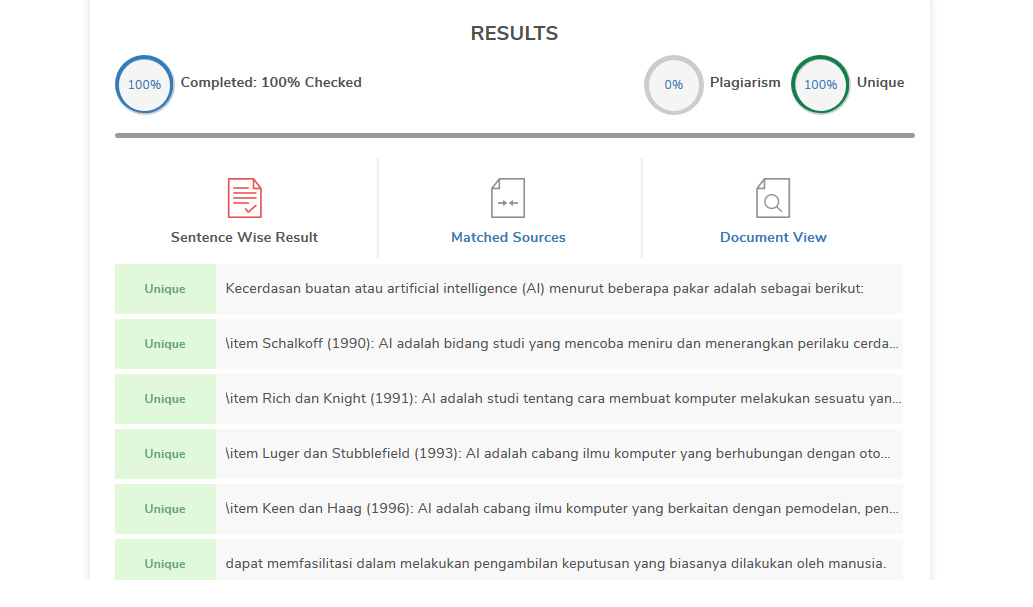
\includegraphics[width=1\textwidth]{figures/chapter1/plagiat.PNG}
	\centering
	\caption{Bukti Tidak Plagiat.}
\end{figure}
\chapter{Membangun Model Prediksi}
\section{Teori}

\subsection{Binary Classification}

\par Setiap data dalam klasifikasi biner memiliki atribut kelas yang berisi dua nilai. Nilai suatu kelas dapat dinyatakan sebagai positif atau negatif. 0 atau 1; benar atau salah; dll. Contoh klasifikasi biner: pemfilteran spam (model klasifikasi yang mendeteksi apakah email diklasifikasikan sebagai spam atau non-spam).\cite{binary}

\begin{figure}[H]
    \centering
    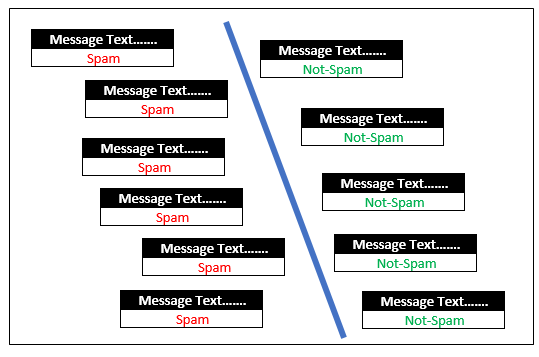
\includegraphics[width=12cm]{figures/chapter2/1.png}
    \caption{Contoh Spam Filtering, Garis Miring Biru adalah class boundary}
\end{figure}

\subsection{Supervised Learning, Unsupervised Learning, dan Clustering}

\par Supervised Learning biasanya digunakan untuk menyelesaikan masalah klasifikasi dan regresi. Algoritma sangat bergantung pada penerapan input dan output pada kumpulan data tertentu, jadi kami (pengguna / ilmuwan data) memainkan peran utama dalam memverifikasi input dan output ini. Perhatikan gambar berikut.

\begin{figure}[H]
    \centering
    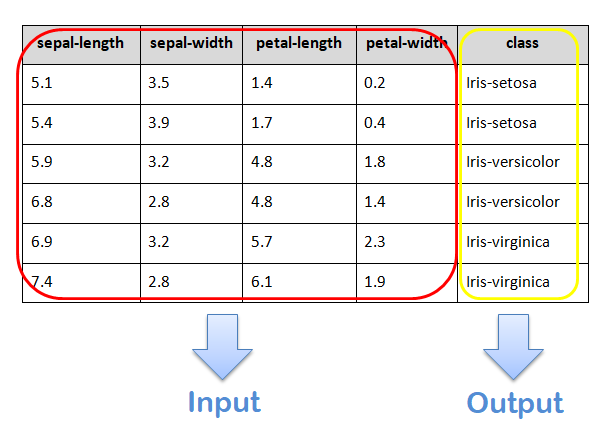
\includegraphics[width=12cm]{figures/chapter2/2.png}
    \caption{Supervised Learning: Dataset Iris}
\end{figure}

\par Pada gambar di atas, input merupakan variabel yang akan diamati, lalu output adalah hasilnya. Dataset iris telah memiliki kategori yang menjadi class, jika kita memasukkan input baru akan keluar hasil sesuai dengan kategori, pada contoh di atas keluar kategori iris-setosa.

\par Unsupervised Learning berarti tidak mengawasi dan memandu model machine learning, tetapi membiarkan model tersebut belajar dengan sendirinya untuk menemukan informasi yang mungkin tidak terlihat oleh mata manusia. Perhatikan gambar berikut.

\begin{figure}[H]
    \centering
    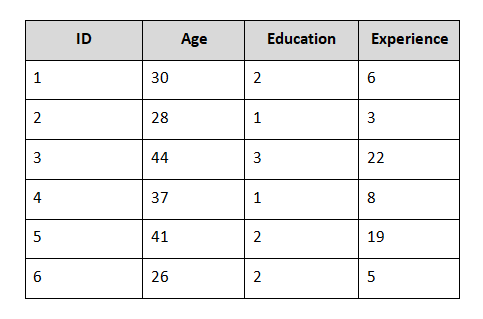
\includegraphics[width=12cm]{figures/chapter2/3.png}
    \caption{Unsupervised Learning}
\end{figure}

\par Seperti yang dapat dilihat dari contoh data di atas, data yang diberikan hanya berupa variabel masukan, tanpa label (Output). Dalam hal ini, model berlatih pada kumpulan data, kemudian mencari informasi dan menarik kesimpulannya sendiri dari data tersebut.

\par Clustering atau pengelompokan merupakan salah satu masalah dalam penggunaan teknik unsupervised learning. Contoh cluster termasuk segmentasi perbankan pelanggan atau segmentasi berita online.

\par Pada dasarnya, jika kumpulan data tidak memiliki label class, teknik unsupervised learning akan digunakan. Dengan kata lain, algoritma dapat secara otomatis membagi data menjadi beberapa cluster berdasarkan kriteria tertentu (seperti kesamaan).\cite{learning}

\subsection{Evaluasi dan Akurasi}

\begin{figure}[H]
    \centering
    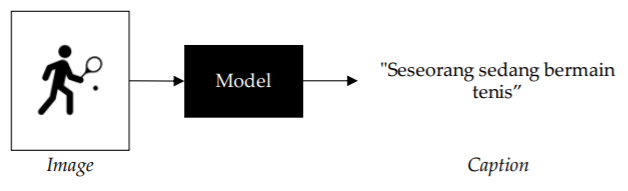
\includegraphics[width=12cm]{figures/chapter2/4.PNG}
    \caption{Model Evaluasi}
\end{figure}

\par Pada gambar di atas, bagaimana Anda mengevaluasi apakah model dapat memberikan penjelasan yang mencerminkan situasi gambar? Misalnya, jika gambar diberikan "Seseorang sedang bermain tenis" dan model memprediksi "Seseorang bermain bola basket", model memberikan interpretasi yang salah. Namun, jika Anda melihat proporsi dari jumlah kata yang sama, Anda berharap ada banyak kata di output yang cocok dengan prediksi, yaitu "seseorang sedang bermain".\cite{evaaku}

\par Akurasi adalah indikator kinerja paling sederhana dan sering digunakan saat mengevaluasi kinerja model. Akurasi didefinisikan sebagai proporsi prediksi yang benar dibagi dengan jumlah sampel. Mengingat output yang diperlukan (juga dikenal sebagai "gold standard") y dan hasil prediksi ˆy, dengan menghitung rasio jumlah elemen yang sama antara y dan ˆy. Secara matematis akurasi dirumuskan dengan persamaan, dimana N merepresentasikan jumlah sampel.\cite{evaaku}

\begin{figure}[H]
    \centering
    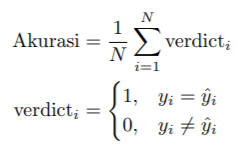
\includegraphics[width=12cm]{figures/chapter2/5.PNG}
    \caption{Akurasi}
\end{figure}

\subsection{Confusion Matrix}

\par Confusion Matrix juga biasa disebut sebagai Error Matrix. Pada dasarnya, confusion matrix memberikan informasi tentang perbandingan hasil klasifikasi yang dilakukan oleh sistem (model) dengan hasil klasifikasi yang sebenarnya. Matriks konfusi berbentuk tabel matriks yang mendeskripsikan performa model klasifikasi pada rangkaian data uji dengan nilai sebenarnya yang diketahui. Gambar di bawah ini adalah matriks konfusi, yang berisi 4 kombinasi berbeda dari nilai prediksi dan nilai aktual. Lihatlah gambar di bawah ini:\cite{matrix}

\begin{figure}[H]
    \centering
    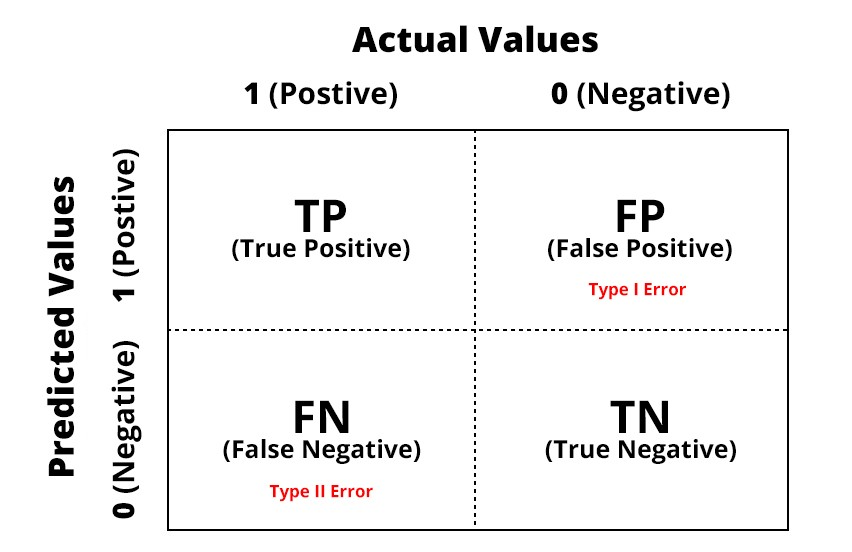
\includegraphics[width=12cm]{figures/chapter2/6.jpeg}
    \caption{Confusion Matrix}
\end{figure}

\begin{itemize}
    \item True Positive (TP)
    \par Ini adalah data positif yang prediksinya benar. Misalnya, pasien menderita kanker (tingkat 1), dan model memprediksi bahwa pasien menderita kanker (tingkat 1).
    \item True Negative (TN)
    \par Menunjukkan data negatif yang diperkirakan benar. Misalnya, pasien tidak mengidap kanker (level 2), dan model memprediksi bahwa pasien tidak mengidap kanker (level 2).
    \item False Postive (FP) — Type I Error
    \par Ini adalah angka negatif, tetapi ramalannya adalah angka positif. Misalnya pasien tidak menderita kanker (kategori 2), tetapi model yang memprediksi bahwa pasien tersebut menderita kanker (kategori 1).
    \item False Negative (FN) — Type II Error
    \par Ini adalah angka positif, tetapi ramalannya adalah angka negatif. Misalnya, seorang pasien mengidap kanker (grade 1), tetapi model memprediksi bahwa pasien tersebut tidak mengidap kanker (grade 2).
\end{itemize}

\subsection{K-Fold Cross Validation}

\par K-fold cross validation merupakan teknik verifikasi dalam pengembangan model verifikasi terpisah, dimana verifikasi mengukur training error dengan menggunakan data uji atau test data untuk pengujian. Pengembangan cross validation sendiri dikarenakan terdapat kelemahan pada model sebelumnya yaitu sampel dipilih secara random, sehingga test error sampling tidak dapat menetapkan kelas secara terstruktur. Walaupun hasil yang didapat dapat dimaksimalkan, tes yang lebih efektif tidak dapat dicapai. Kemudian muncul cross validation, yang dapat bekerja dengan cepat dengan pengambilan sampel yang lebih terstruktur. Oleh karena itu, meskipun dalam jumlah pengujian, data yang berbeda dari eksperimen atau literasi sebelumnya akan digunakan untuk mendapatkan beberapa training dataset dan testing dataset.\cite{cross}

\begin{figure}[H]
    \centering
    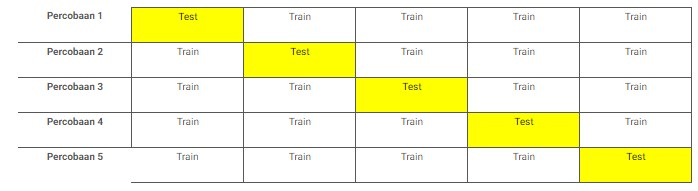
\includegraphics[width=12cm]{figures/chapter2/7.jpg}
    \caption{5-Fold Cross Validation}
\end{figure}

\par Percobaan di atas merupakan contoh validasi silang 5 kali lipat, yang artinya percobaan tersebut perlu dilakukan 5 tahap. Percobaan 1, untuk mengubah bagian pertama dari partisi menjadi data test, dan partisi lainnya menjadi data training, dan seterusnya. 

\par Dari 5 hasil percobaan ini, kita akan menggunakan confusion matrix untuk mencatat nilai evaluasi kinerja model, kemudian menentukan nilai rata-rata setiap percobaan. Kemudian, akan ditemukan eksperimen mana yang dapat digunakan sebagai referensi untuk menggunakan model algoritma yang dipilih.

\subsection{Decision Tree}

\begin{figure}[H]
    \centering
    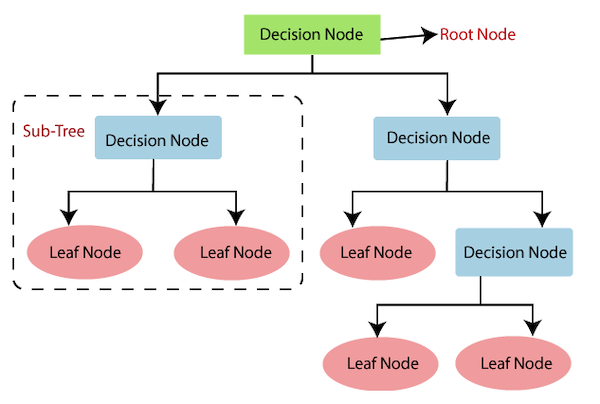
\includegraphics[width=12cm]{figures/chapter2/8.png}
    \caption{5-Fold Cross Validation}
\end{figure}

\par Decision Tree adalah diagram yang dapat membantu Anda memilih salah satu dari beberapa opsi pengoperasian. Biasanya, dimulai dengan satu atau lebih node. Kemudian, cabang node menunjukkan opsi yang tersedia. Selain itu, setiap cabang tersebut akan memiliki cabang baru. Oleh karena itu, cara ini dinamakan "Tree" karena mirip dengan pohon yang banyak cabangnya. Decision tree dapat membuat berbagai pilihan dan menyelidiki kemungkinan hasil dari pilihan tersebut. Selain itu, Anda juga dapat melihat potensi risiko dan keuntungan dari setiap opsi. Mengutip dari Venngage, decision tree mengandung tiga unsur, yaitu:\cite{tree}

\begin{itemize}
    \item Root Node (Akar): tujuan akhir atau keputusan besar yang harus dibuat.
    \item Branches (Ranting): berbagai opsi tindakan.
    \item Leaf Node (Daun): kemungkinan hasil atas setiap opsi tindakan.
\end{itemize}

\subsection{Entropi dan Information Gain}

\par Pohon keputusan dibangun dari simpul akar dari atas ke bawah dan melibatkan pembagian data menjadi subset yang berisi contoh nilai yang sama (homogen). Algoritma ID3 menggunakan entropi untuk menghitung keseragaman sampel. Jika sampel benar-benar seragam, entropinya nol; jika distribusi sampel sama, entropi adalah 1.\cite{entropi}

\begin{figure}[H]
    \centering
    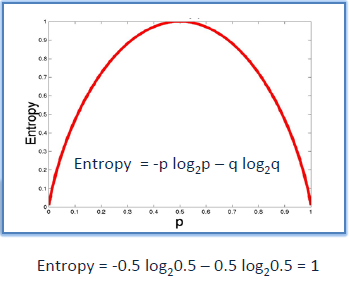
\includegraphics[width=12cm]{figures/chapter2/9.png}
    \caption{Entrophy}
\end{figure}

\begin{enumerate}
    \item Entropi yang menggunakan tabel frekuensi atribut tunggal:
    \begin{figure}[H]
        \centering
        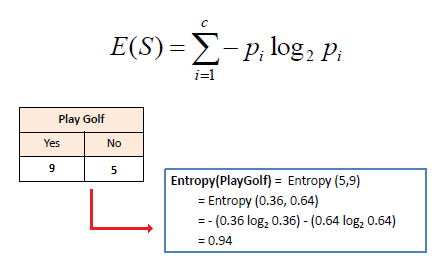
\includegraphics[width=12cm]{figures/chapter2/10.png}
        \caption{Entrophy Atribut Tunggal}
    \end{figure}
    \item Entropi yang menggunakan tabel frekuensi dua atribut:
    \begin{figure}[H]
        \centering
        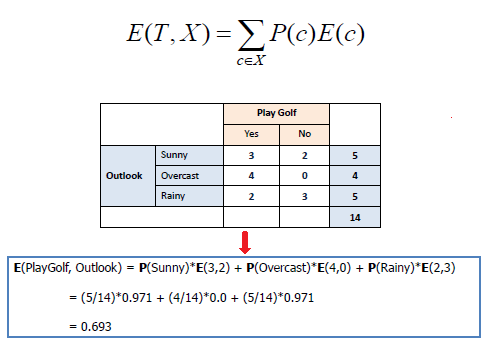
\includegraphics[width=12cm]{figures/chapter2/11.png}
        \caption{Entrophy Dua Atribut}
    \end{figure}
\end{enumerate}

\par Information gain didasarkan pada pengurangan entropi setelah kumpulan data dibagi dengan atribut. Keseluruhan proses membangun pohon keputusan adalah menemukan atribut yang mengembalikan perolehan informasi tertinggi (yaitu, cabang yang paling homogen).

\begin{enumerate}
    \item Langkah Pertama: Hitung Entropi.
    \begin{figure}[H]
        \centering
        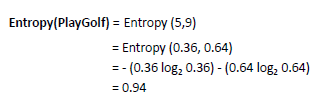
\includegraphics[width=12cm]{figures/chapter2/12.png}
        \caption{Langkah 1}
    \end{figure}
    \item Langkah 2: Kemudian bagi kumpulan data menjadi atribut yang berbeda. Hitung entropi setiap cabang. Kemudian tambahkan secara proporsional untuk mendapatkan nilai entropi dari pembagian tersebut. Kurangi entropi yang dihasilkan dari entropi sebelum pemisahan. Hasilnya adalah penurunan perolehan informasi atau entropi.
    \begin{figure}[H]
        \centering
        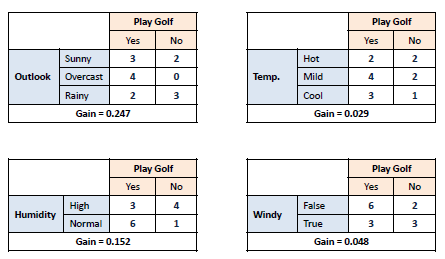
\includegraphics[width=12cm]{figures/chapter2/13.png}
    \end{figure}
    \begin{figure}[H]
        \centering
        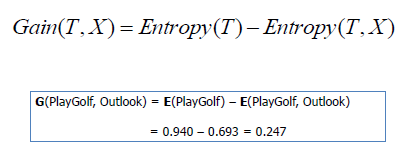
\includegraphics[width=12cm]{figures/chapter2/14.png}
        \caption{Langkah 2}
    \end{figure}
    \item Langkah 3: Pilih atribut dengan perolehan informasi terbesar sebagai simpul keputusan, bagi kumpulan data menjadi beberapa cabang, dan ulangi proses yang sama pada setiap cabang.
    \begin{figure}[H]
        \centering
        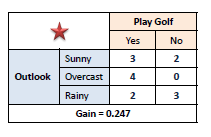
\includegraphics[width=12cm]{figures/chapter2/15.png}
    \end{figure}
    \begin{figure}[H]
        \centering
        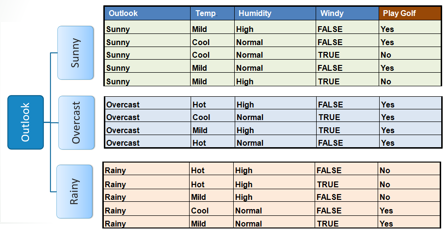
\includegraphics[width=12cm]{figures/chapter2/16.png}
        \caption{Langkah 3}
    \end{figure}
    \item Langkah 4a: Cabang dengan entropi 0 adalah simpul daun.
    \begin{figure}[H]
        \centering
        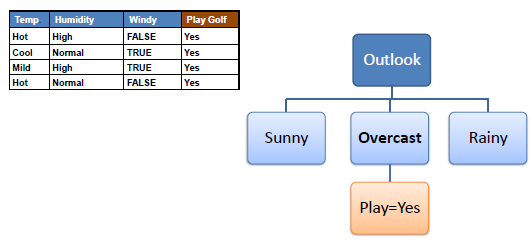
\includegraphics[width=12cm]{figures/chapter2/17.png}
        \caption{Langkah 4a}
    \end{figure}
    \item Langkah 4b: Cabang dengan entropi lebih besar dari 0 akan dipecah lagi.
    \begin{figure}[H]
        \centering
        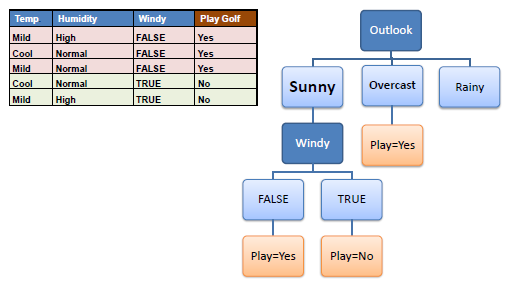
\includegraphics[width=12cm]{figures/chapter2/18.png}
        \caption{Langkah 4b}
    \end{figure}
\end{enumerate}

\section{Scikit Learn}

\par Dataset ambil di https://github.com/PacktPublishing/Python-Artificial-Intelligence-Projects-for-Beginners folder Chapter01. Tugas anda adalah, dataset ganti menggunakan student-mat.csv dan mengganti semua nama variabel dari kode di bawah ini dengan nama-nama makanan (NPM mod 3=0), kota (NPM mod 3=1), buah (NPMmod 3=2).

\subsection{Nomor 1}
\begin{lstlisting}[language=Python]
import pandas as pd #import library pandas dengan alias pd
akiba = pd.read_csv('D:/[Matkul]/AI/Chapter 2/Python-Artificial-Intelligence-Projects-for-Beginners-master/Chapter01/dataset/student-mat.csv', sep=';') #sebuah variable akiba untuk memanggil file csv
len(akiba) #untuk menghitung jumlah data di file csv
\end{lstlisting}

\par Hasilnya:

\begin{figure}[H]
    \centering
    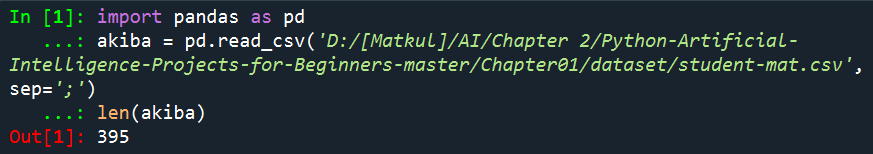
\includegraphics[width=12cm]{figures/chapter2/19.PNG}
    \caption{Nomor 1}
\end{figure}

\subsection{Nomor 2}

\begin{lstlisting}[language=Python]
akiba['pass'] = akiba.apply(lambda row: 1 if (row['G1']+row['G2']+row['G3'])>= 35 else 0, axis=1) #membuat label binary pass atau fail berdasarkan G1G2G3 dengan batas data lebih atau sama dengan 35
akiba = akiba.drop(['G1', 'G2', 'G3'], axis=1) #menghitung G1,2,3
akiba.head() #menampilkan data
\end{lstlisting}

\par Hasilnya

\begin{figure}[H]
    \centering
    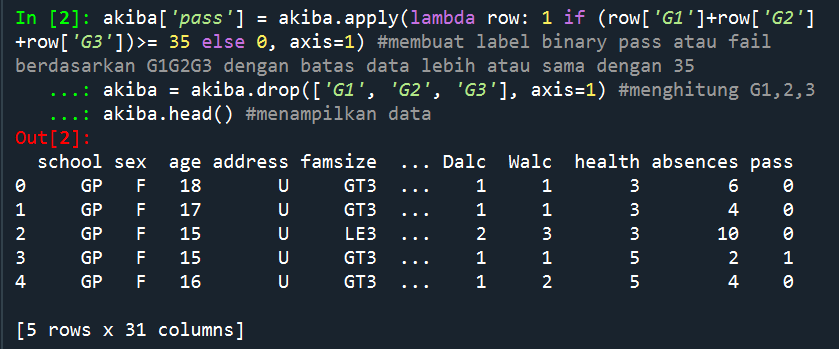
\includegraphics[width=12cm]{figures/chapter2/20.PNG}
    \caption{Nomor 2}
\end{figure}

\subsection{Nomor 3}

\begin{lstlisting}[language=Python]
#memanggil kolom pada file csv
akiba = pd.get_dummies(akiba, columns=['sex', 'school', 'address', 'famsize', 'Pstatus', 'Mjob',
                                       'Fjob', 'reason', 'guardian', 'schoolsup', 'famsup', 'paid',
                                       'activities', 'nursery', 'higher', 'internet', 'romantic'])
akiba.head() #menampilkan data
\end{lstlisting}

\par Hasilnya

\begin{figure}[H]
    \centering
    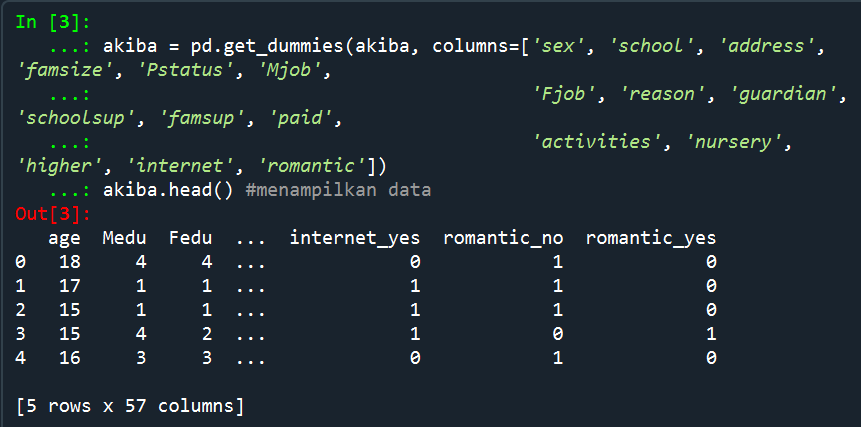
\includegraphics[width=12cm]{figures/chapter2/21.PNG}
    \caption{Nomor 3}
\end{figure}

\subsection{Nomor 4}

\begin{lstlisting}[language=Python]
akiba = akiba.sample(frac=1) #variable akiba dengan isi data sample
akiba_train = akiba[:500] #membagi data untuk training
akiba_test = akiba[500:] #membagi data untuk test

akiba_train_att = akiba_train.drop(['pass'], axis=1) #menghapus data yang telah lewat(pass) kemudian diinputkan
akiba_train_pass = akiba_train['pass'] #mengambil data pass saja

akiba_test_att = akiba_test.drop(['pass'], axis=1) #menghapus data yang telah lewat(pass) kemudian diinputkan
akiba_test_pass = akiba_test['pass'] #mengambil data pass saja

akiba_att = akiba.drop(['pass'], axis=1) #menghapus data yang telah lewat(pass) kemudian diinputkan
akiba_pass = akiba['pass'] #mengambil data pass saja

import numpy as np #import library numpy dengan alias np
print ("Passing: %a out of %a (%.2f%%)" % (np.sum(akiba_pass), len(akiba_pass), 100*float(np.sum(akiba_pass)) / len(akiba_pass))) #menampilkan data
\end{lstlisting}

\par Hasilnya

\begin{figure}[H]
    \centering
    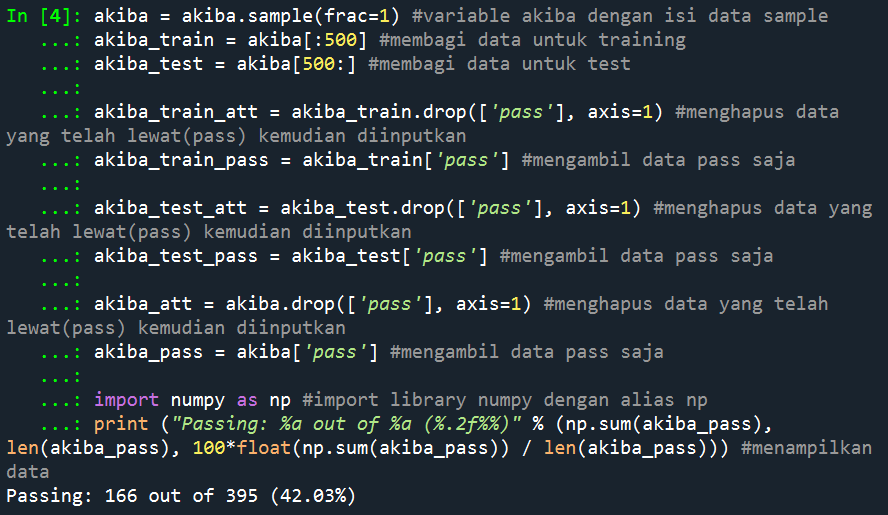
\includegraphics[width=12cm]{figures/chapter2/22.PNG}
    \caption{Nomor 4}
\end{figure}

\subsection{Nomor 5}

\begin{lstlisting}[language=Python]
from sklearn import tree #import library tree dari sklearn
tokyo = tree.DecisionTreeClassifier(criterion="entropy", max_depth=5) #membuat decision tree dengan max depth adalah 5
tokyo = tokyo.fit(akiba_train_att, akiba_train_pass) #memasukkan data untuk decision tree
\end{lstlisting}

\par Hasilnya

\begin{figure}[H]
    \centering
    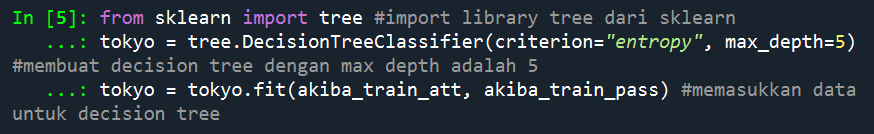
\includegraphics[width=12cm]{figures/chapter2/23.PNG}
    \caption{Nomor 5}
\end{figure}

\subsection{Nomor 6}

\begin{lstlisting}[language=Python]
import graphviz #import library graphviz
dot_data = tree.export_graphviz(tokyo, out_file=None, label="all", impurity=False, 
                                proportion=True, feature_names=list(akiba_train_att), 
                                class_names=["fail", "pass"], filled=True, rounded=True) #mendefinisikan data yang akan divisualisasikan di decision tree
graph = graphviz.Source(dot_data) #memasukkan data ke variable graph
graph #menampilkan gambar
\end{lstlisting}

\par Hasilnya

\begin{figure}[H]
    \centering
    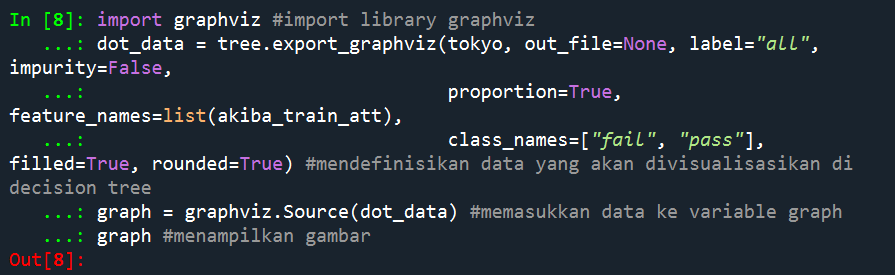
\includegraphics[width=12cm]{figures/chapter2/24.PNG}
    \caption{Nomor 6}
\end{figure}

\par visualisasi decision tree

\begin{figure}[H]
    \centering
    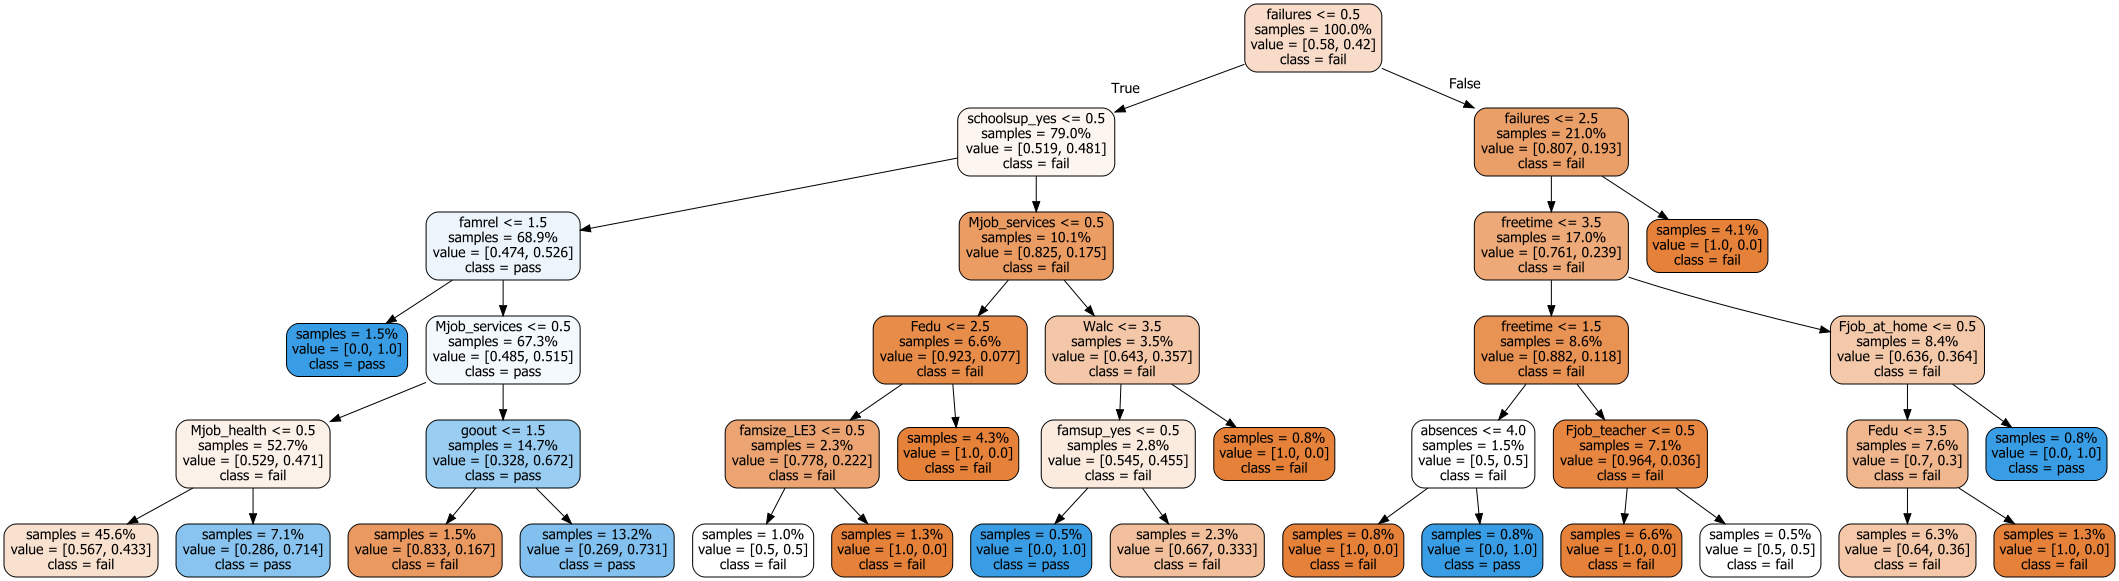
\includegraphics[width=12cm]{figures/chapter2/25.png}
    \caption{Nomor 6}
\end{figure}

\subsection{Nomor 7}

\begin{lstlisting}[language=Python]
tree.export_graphviz(tokyo, out_file="student-performance.dot",
                     label="all", impurity=False,
                     proportion=True,
                     feature_names=list(akiba_train_att),
                     class_names=["fail", "pass"],
                     filled=True, rounded=True) #untuk ekspor graph decision tree
\end{lstlisting}

\par Hasilnya

\begin{figure}[H]
    \centering
    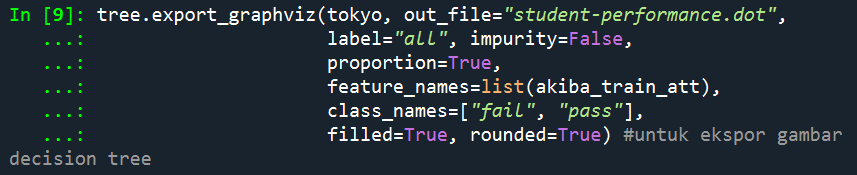
\includegraphics[width=12cm]{figures/chapter2/26.PNG}
    \caption{Nomor 7}
\end{figure}

\par Lokasi file student-performance.dot pada komputer, dapat diliat yang ditandai biru.

\begin{figure}[H]
    \centering
    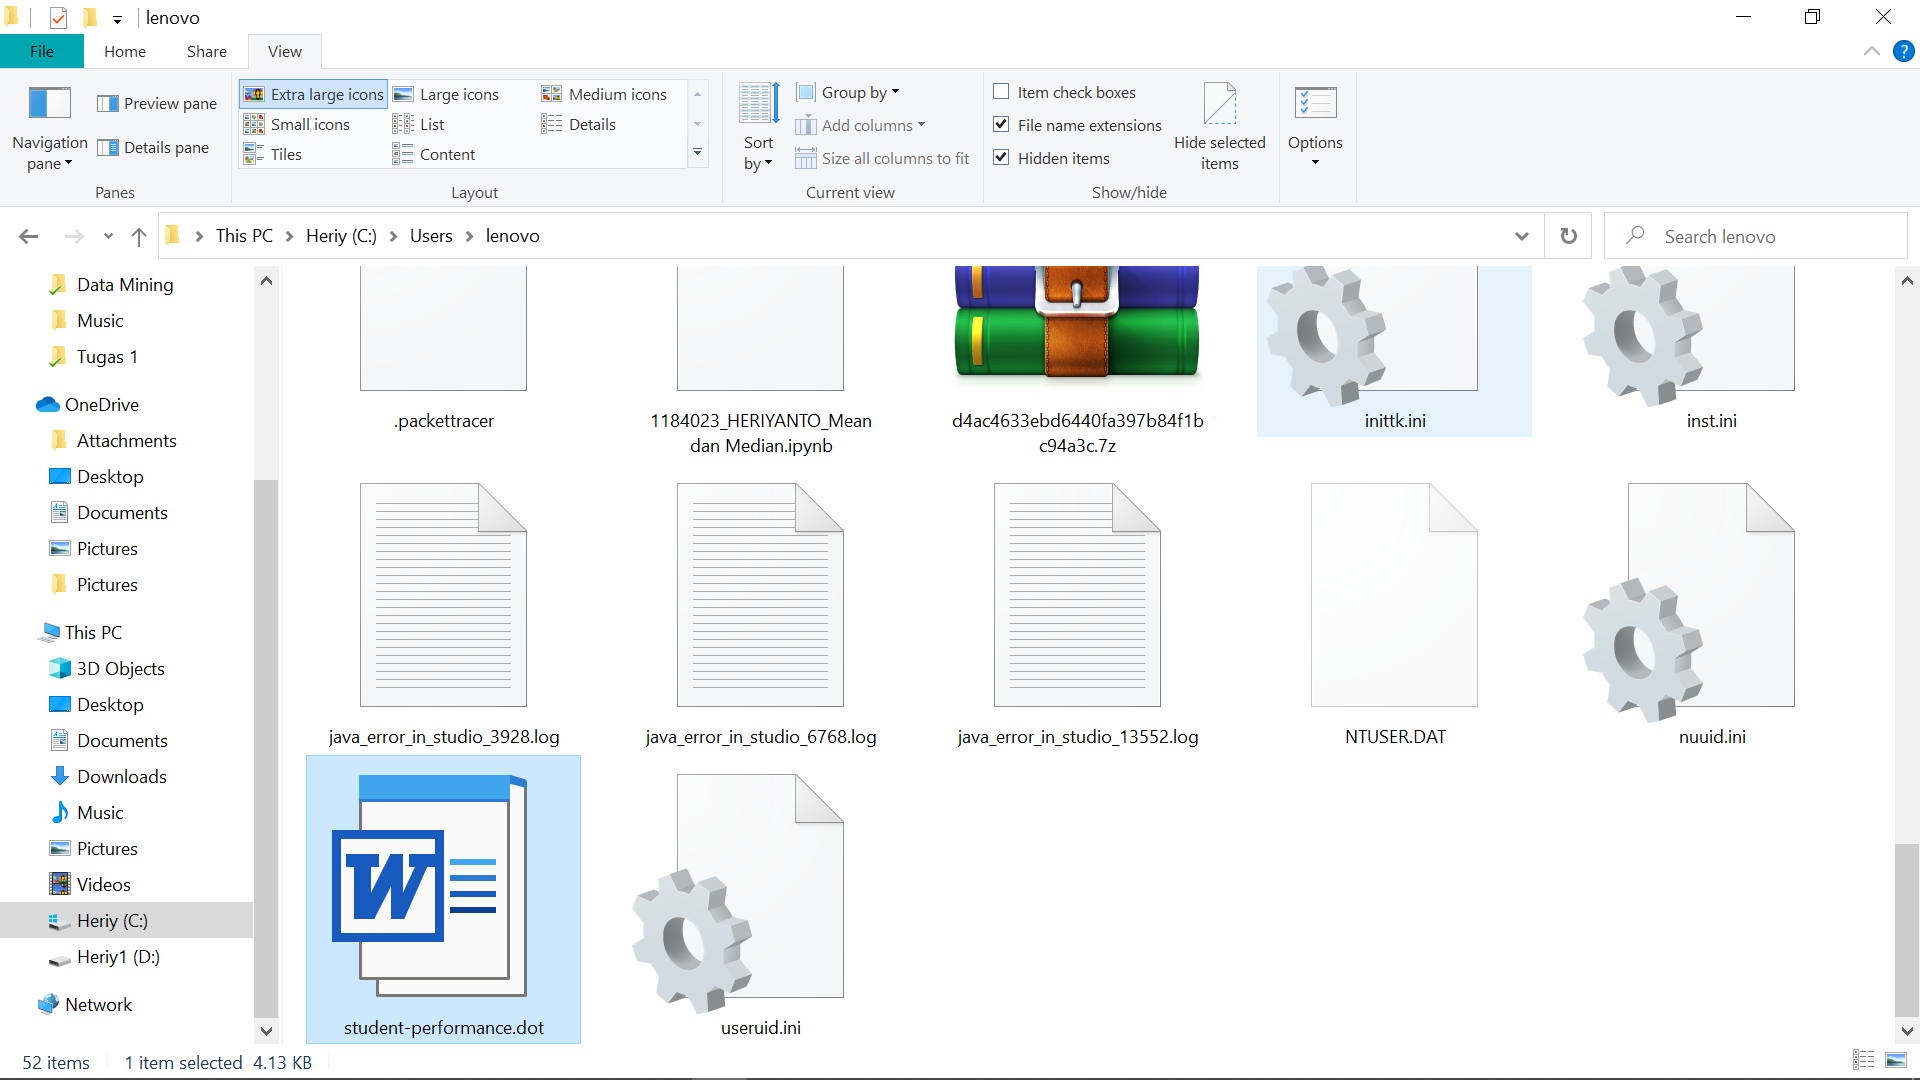
\includegraphics[width=12cm]{figures/chapter2/27.PNG}
    \caption{Nomor 7}
\end{figure}

\subsection{Nomor 8}

\begin{lstlisting}[language=Python]
tokyo.score(akiba_test_att, akiba_test_pass) #menghitung prediksi nilai yang akan datang
\end{lstlisting}

\par Hasilnya error, kenapa hasilnya error karena hasil prediksi dari student-mat.csv itu nol(0), jadi tidak menampilkan nilai prediksi. Untuk menampilkan nilai prediksi minimal nilainya harus 1.

\begin{figure}[H]
    \centering
    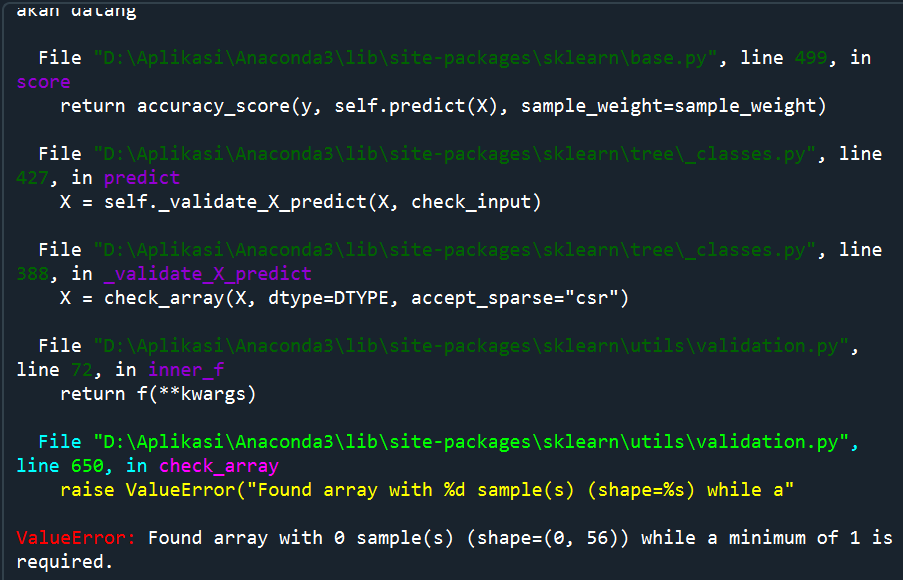
\includegraphics[width=12cm]{figures/chapter2/28.PNG}
    \caption{Nomor 8}
\end{figure}

\subsection{Nomor 9}

\begin{lstlisting}[language=Python]
from sklearn.model_selection import cross_val_score #import module cross_val_score dari sklearn.model_selection
okinawa = cross_val_score(tokyo, akiba_att, akiba_pass, cv=5) #pembagian data menjadi 5 bagian
print ("Accuracy: %0.2f (+/- %0.2f)" % (okinawa.mean(), okinawa.std() * 2)) #menampilkan hasil dari rata-rata dan standar deviasi dikali 2
\end{lstlisting}

\par Hasilnya

\begin{figure}[H]
    \centering
    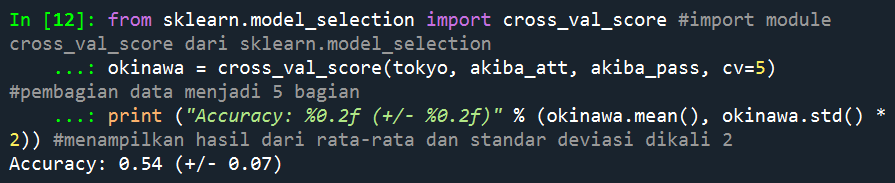
\includegraphics[width=12cm]{figures/chapter2/29.PNG}
    \caption{Nomor 9}
\end{figure}

\subsection{Nomor 10}

\begin{lstlisting}[language=Python]
for max_depth in range(1, 20): #pengulangan max depth dalam jangkauan 1-20
    tokyo = tree.DecisionTreeClassifier(criterion="entropy", max_depth=max_depth) #membuat decision tree 
    okinawa = cross_val_score(tokyo, akiba_att, akiba_pass, cv=5) #pembagian data menjadi 5 bagian
    print("Max depth: %d, Accuracy: %0.2f (+/- %0.2f)" % (max_depth, okinawa.mean(), okinawa.std() * 2)) #menampilkan hasil dari rata-rata dan standar deviasi dikali 2
\end{lstlisting}

\par Hasilnya

\begin{figure}[H]
    \centering
    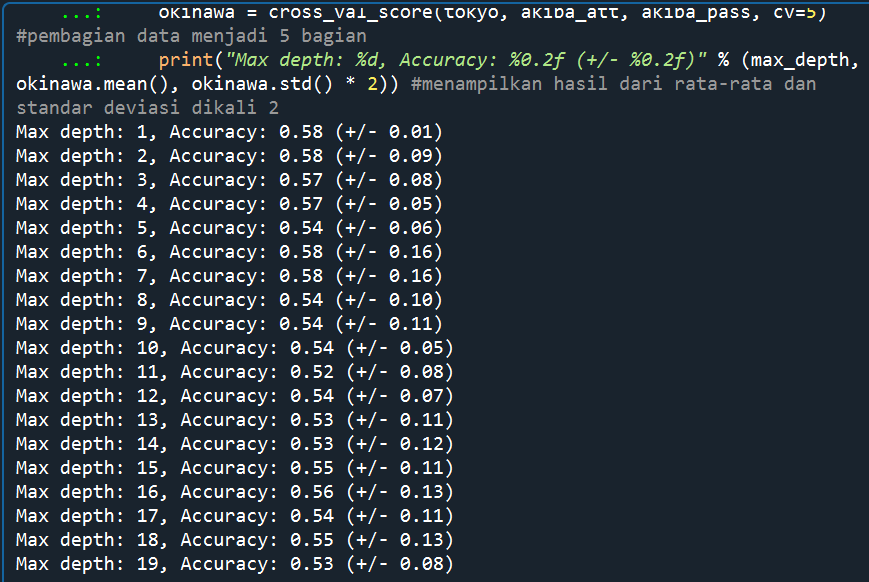
\includegraphics[width=12cm]{figures/chapter2/30.PNG}
    \caption{Nomor 10}
\end{figure}

\subsection{Nomor 11}

\begin{lstlisting}[language=Python]
depth_acc = np.empty((19,3), float) #membuat array baru
i = 0 #variable i dengan isi 0
for max_depth in range(1, 20): #pengulangan dalam jangkauan 1-20
    tokyo = tree.DecisionTreeClassifier(criterion="entropy", max_depth=max_depth) #membuat decision tree
    okinawa = cross_val_score(tokyo, akiba_att, akiba_pass, cv=5) #pembagian data menjadi 5 bagian 
    depth_acc[i,0] = max_depth #meng-inputkan data max depth ke array depth acc
    depth_acc[i,1] = okinawa.mean() #meng-inputkan rata-rata ke array depth acc 
    depth_acc[i,2] = okinawa.std() * 2 #meng-inputkan nilai standar deviasi ke array depth acc
    i += 1

depth_acc
\end{lstlisting}

\begin{figure}[H]
    \centering
    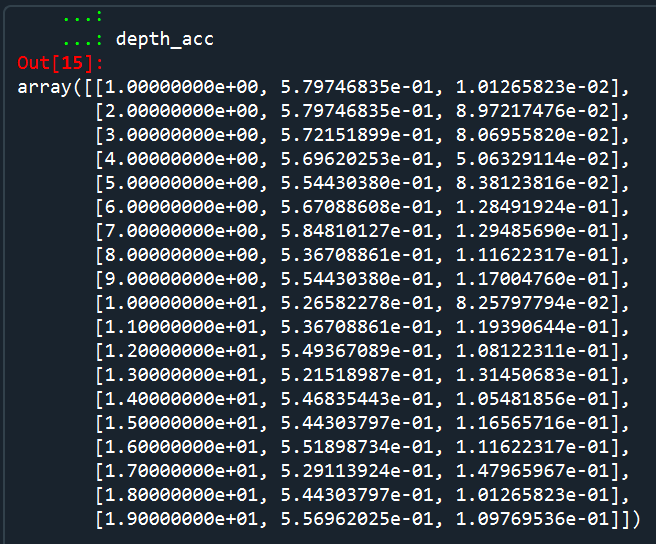
\includegraphics[width=12cm]{figures/chapter2/31.PNG}
    \caption{Nomor 11}
\end{figure}

\subsection{Nomor 12}

\begin{lstlisting}[language=Python]
import matplotlib.pyplot as plt #import library matplotlib dengan alias plt
fig, ax = plt.subplots() #membuat plot baru
ax.errorbar(depth_acc[:,0], depth_acc[:,1], yerr=depth_acc[:,2]) #mengisi data plot
plt.show() #menampilkan data plot
\end{lstlisting}

\begin{figure}[H]
    \centering
    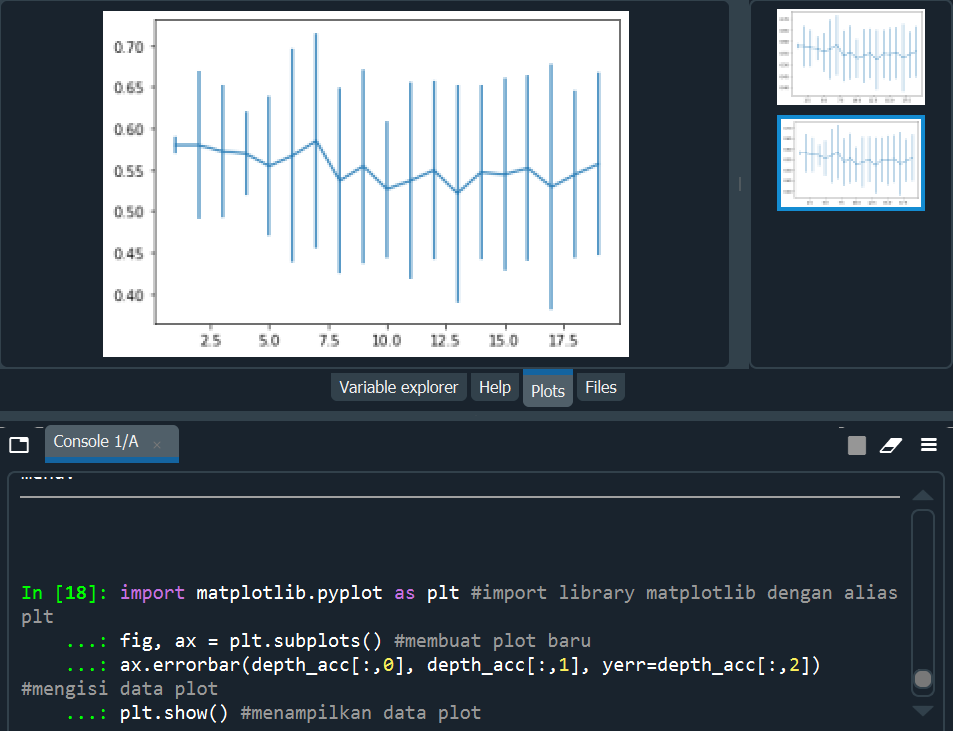
\includegraphics[width=12cm]{figures/chapter2/32.PNG}
    \caption{Nomor 12}
\end{figure}
% \include{section/chapter3}
% \include{section/chapter4}
% \include{section/chapter5}
% \include{section/chapter6}
% \include{section/chapter7}
% \include{section/chapter8}
% \include{section/chapter9}
% \include{section/chapter10}
% \include{section/chapter11}
% \include{section/chapter12}
% \include{section/chapter13}
% \include{section/chapter14}

%now enable appendix numbering format and include any appendices
% \appendix
% \chapter{Form Penilaian Jurnal}

gambar \ref{form1} dan \ref{form2} merupakan contoh bagaimana reviewer menilai jurnal kita. 
\begin{figure}[ht]
      \centerline{\includegraphics[width=1\textwidth]
      {figures/form1}}
      \caption{Form nilai bagian 1.}
      \label{form1}
      \end{figure}

	\begin{figure}[ht]
	      \centerline{\includegraphics[width=1\textwidth]
	      {figures/form2}}
	      \caption{form nilai bagian 2.}
	      \label{form2}
	      \end{figure}

% \chapter{FAQ}

M : Kalo Intership II atau TA harus buat aplikasi ?
D : Ga harus buat aplikasi tapi harus ngoding

M : Pa saya bingung mau ngapain, saya juga bingung mau presentasi apa?
D : Makanya baca de, buka jurnal topik `ganteng' nah kamu baca dulu sehari 5 kali ya, 4 hari udah 20 tuh. Bingung itu tanda kurang wawasan alias kurang baca.

M : Pa saya sudah cari jurnal terindeks scopus tapi ga nemu.
D : Kamu punya mata de? coba dicolok dulu. Kamu udah lakuin apa aja? tolong di list laporkan ke grup Tingkat Akhir. Tinggal buka google scholar klik dari tahun 2014, cek nama jurnalnya di scimagojr.com beres.

M : Pa saya belum dapat tempat intership, jadi ga tau mau presentasi apa?
D : kamu kok ga nyambung, yang dipresentasikan itu yang kamu baca bukan yang akan kamu lakukan.

M : Pa ini jurnal harus yang terindex scopus ga bisa yang lain ?
D : Index scopus menandakan artikel tersebut dalam standar semantik yang mudah dipahami dan dibaca serta bukan artikel asal jadi. Jika diluar scopus biasanya lebih sukar untuk dibaca dan dipahami karena tidak adanya proses review yang baik dan benar terhadap artikel.

M : Pa saya tidak mengerti
D : Coba lihat standar alasan

M : Pa saya bingung
D : Coba lihat standar alasan

M : Pa saya sibuk
D : Mbahmu....

M : Pa saya ganteng
D : Ndasmu....

M : Pa saya kece
D : wes karepmu lah....


Biasanya anda memiliki alasan tertentu jika menghadapi kendala saat proses bimbingan, disini saya akan melakukan standar alasan agar persepsi yang diterima sama dan tidak salah kaprah. Penggunaan kata alasan tersebut antara lain :

1. Tidak Mengerti : anda boleh menggunakan alasan ini jika anda sudah melakukan tahapan membaca dan meresumekan 15 jurnal. Sudah mencoba dan mempraktekkan teorinya dengan mencari di youtube dan google minimal 6 jam sehari selama 3 hari berturut-turut.

2. Bingung : anda boleh mengatakan alasan bingung setelah maksimal dalam berusaha menyelesaikan tugas bimbingan dari dosen(sudah dilakukan semua). Anda belum bisa mengatakan alasan bingung jika anda masih belum menyelesaikan tugas bimbingan dan poin nomor 1 diatas. Setelah anda menyelesaikan tugas bimbingan secara maksimal dan tahap 1 poin diatas, tapi anda masih tetap bingung maka anda boleh memakai alasan ini.

%next line adds the Bibliography to the contents page
\addcontentsline{toc}{chapter}{Bibliography}
%uncomment next line to change bibliography name to references
%\renewcommand{\bibname}{References}
\bibliography{references}        %use a bibtex bibliography file refs.bib
\bibliographystyle{plain}  %use the plain bibliography style

\end{document}

